\documentclass[10pt]{article}
\usepackage[letterpaper,margin=0.2in]{geometry}
\usepackage{amsmath,amssymb,bm}
\newcommand{\ind}{\mathbb{I}}
\usepackage{multicol}
\usepackage{graphicx}
\usepackage{enumitem}
\usepackage{titlesec}

\setlength{\parindent}{0pt}
\setlength{\columnsep}{8pt}
\setlength{\columnseprule}{0.2pt}
\setlist{nosep,leftmargin=*}
\titleformat*{\section}{\large\bfseries}
\titleformat*{\subsection}{\normalsize\bfseries}
\titlespacing*{\section}{0pt}{3pt}{1pt}
\titlespacing*{\subsection}{0pt}{2pt}{0pt}
\AtBeginDocument{\setlength{\abovedisplayskip}{2pt}\setlength{\belowdisplayskip}{2pt}\setlength{\abovedisplayshortskip}{0pt}\setlength{\belowdisplayshortskip}{1pt}}
\setlength{\jot}{1pt}
\pagestyle{empty}

\newcommand{\vx}{\mathbf{x}}
\newcommand{\vw}{\mathbf{w}}
\newcommand{\vt}{\mathbf{t}}
\newcommand{\vu}{\mathbf{u}}
\newcommand{\vv}{\mathbf{v}}
\newcommand{\vr}{\mathbf{r}}
\newcommand{\cE}{\mathcal{E}}
\newcommand{\cL}{\mathcal{L}}

\begin{document}
\fontsize{9.5}{11}\selectfont
\begin{multicols*}{3}

\section{KNN}
\subsection{The Very Basics}
\textbf{Learning}: find a model $f$ that maps from inputs to outputs given a labeled training dataset.\\
\textbf{Inference}: use a model $f$ to predict an output $y$ given a new example $\vec{x}$\\
\textbf{A model} is a function $f$ mapping input $\vec{x}$ to output prediction $y$.\\
\textbf{A model family} is a set of models that share the same structure but differ in parameters (e.g.\ layers in a neural network)\\
\textbf{Accuracy} is calculated as follows:
\[ \frac{\sum_{i=1}^N \ind\left[t^{(i)}=y^{(i)}\right]}{N} \]
A \textbf{parameter} is the internal variables of a model learned from data whilst training.\\
A \textbf{hyperparameter} are the settings chosen before training that controls how the learning process works.\\
\textbf{Train} fit params; \textbf{Val} tune hyperparams / pick model; \textbf{Test} use once $\to$ unbiased gen.\ error (tune on test $\to$ leakage, optimistic).\\
Reg.\ vs class.\ decided by \emph{output} only (cont.\ vs discrete). $t$=target, $y$=pred; $x^{(i)}_j$: ex.\ $i$, feat.\ $j$.\\
100\% train acc $\not\Rightarrow$ good test; May overfit. Data augmentation: changing the training data by a little bit to create new training data (shift/rotate).\\
\textbf{Parametric models} fix the parameter count. Non-parametric models don't. $\mathcal{O}(1)$ space complexity with respect to the feature count, and never $\Omega(N)$. Hyperparameters are out of this scope.

\subsection{KNN}
For 1NN: Find $t^{(c)}$ that corresponds to:
\[ \vec{x}^{(c)} = \arg\min_{\vec{x}^{(i)}\in\text{training set}} \operatorname{distance}\left(\vec{x}^{(i)},\, \vec{x}\right) \]
For kNN, for the top $k$ other datapoints closest to $\vx$, choose the majority class.\\
{\scriptsize Distances ($\mathbf a,\mathbf b\in\mathbb R^d$):\\
\begin{minipage}[t]{0.5\linewidth}
$L_2$: $\sqrt{\sum_j (a_j-b_j)^2}$\\[1pt]
$L_p$: $\big(\sum_j |a_j-b_j|^p\big)^{1/p}$
\end{minipage}\vrule\hspace{2pt}
\begin{minipage}[t]{0.47\linewidth}
Cos: $\frac{\mathbf a\cdot\mathbf b}{\|\mathbf a\|_2\|\mathbf b\|_2}$\\[1pt]
$L_\infty$: $\max_j |a_j-b_j|$
\end{minipage}}\\
Normalize features to mean $=0$ and var $=1$:
\[ x_{\text{norm}} = \frac{x-\mu}{\sigma} \]
$\mu_j,\sigma_j$ from training set only; Reuse for val/test (else leakage).\\
\textbf{Pros}: simple; No training; Works for reg.\ and class.; Adapts easily to new data.\\
\textbf{Cons}: \textbf{curse of dimensionality}: in high dims most points are far apart from each other ($L_\infty$ on $[0,1]^d$: frac.\ within $\epsilon$ of origin $=\epsilon^d$; $\because\epsilon<1$, $d\uparrow\Rightarrow\epsilon^d\to0$); Sensitive to ranges of features (larger range dominates distance calculations); Slow prediction: distance to all $N$ pts, $O(ND)$ per query; Must store entire training set, $O(ND)$ space.\\
\textbf{Choose $k$}\\
$k\uparrow\ \to$ boundary smoother, less sensitive to individual pts $\to$ underfit; $k=N\to$ always majority class.\\
$k=1\to$ sharp, overfit; 100\% train acc (unless dup.\ $\vx$ w/ diff.\ labels). No single best $k$, depends on $N$; Heuristic $k<\sqrt N$ ($k\to\infty$, $k/N\to0$). Pick $k$ (any hyperparam) via val set or cross-val.\\
\textbf{Workflow}: (1) Split into train/val/test; (2) For each $K$, train KNN on train; (3) Compute acc of each on val; (4) Select $K$ w/ best val acc; (5) Compute acc of that $K$ on test.\\
Cos: direction $>$ magnitude (text). Curse: need exp.\ more data; Nearest $\approx$ farthest dist.; Large $k$ doesn't fix.

\section{Decision Trees}
Large trees overfit, small trees underfit. For inference, trace the tree.\\
\textbf{Entropy}
\[ H(X) = -\textstyle\sum_{x\in X} p(x)\log_2 p(x) \]
\textbf{Conditional Entropy}
\[ H(X\mid Y\!=\!y) = -\textstyle\sum_{x} p(x\mid y)\log_2 p(x\mid y) \]
\textbf{Expected conditional entropy}
\[ H(X\mid Y) = \textstyle\sum_{y} p(y)\,H(X\mid Y\!=\!y) \]
\textbf{Information gain}
\[ IG(X\mid Y) = H(X) - H(X\mid Y) \]
\textbf{Properties}: $H(X)\ge0$; $H(Y\mid X) \le H(Y)$ (i.e.\ $IG\ge0$); $Y, X$ are independent $\Rightarrow IG(Y\mid X) = 0$ (i.e.\ $H(Y\mid X)=H(Y)$); $Y$ fully determined by $X\Rightarrow H(Y\mid X)=0\Rightarrow IG(Y\mid X)=H(Y)$; Certain $\to H=0$; Binary max $H=1$ bit at $p=.5$.\\

\subsection{Decision Tree Algorithm}
Keep splitting until:
\begin{itemize}
  \item All examples have the same label.
  \item When there are no features left.
  \item When a depth limit is reached. (hyperparameter)
  \item When the loss stops decreasing enough. (hyperparameter)
  \item Node has $<$ min \#samples. (hyperparameter)
\end{itemize}
Split: pick max IG (not train error $\because$ ignores child uncertainty). Leaf $\to$ majority class.
Greedy $\to$ not globally optimal ($\because$ NP-hard). Boundaries axis-aligned ($x_j\le\theta$). Continuous feat.: only $\le N\!-\!1$ thresholds (midpts between sorted values). Scale-invariant.

\section{Linear / GD}
Loss function measures how off once training example is.\\
Pred.: $y=\vw^T\vx+b$, $\mathbf y=X\vw$ ($X$: $N\times(D\!+\!1)$, row = example).\\
\textbf{Closed form}: $\nabla=0\Rightarrow X^TX\vw=X^T\vt\Rightarrow\vw=(X^TX)^{-1}X^T\vt$.\\
$\nabla$ = steepest ascent, $\perp$ contours $\to$ step along $-\nabla$. $\alpha$ too big $\to$ overshoot/diverge; Too small $\to$ slow.\\
Feature map $\psi(\vx)$ (e.g.\ $[1,x,x^2]$) $\to$ nonlinear fit, still linear in $\vw$.\\
Reg.\ $\cE+\lambda\mathcal R$: $\lambda$ small $\to$ overfit; Big $\to$ underfit.\\
Cost functions sum up all.
\[ \cL(y,t) = \tfrac{1}{2}(y-t)^2 \]
\[ \cE(\vw) = \tfrac{1}{N}\textstyle\sum_{i=1}^N \cL\left(y^{(i)}, t^{(i)}\right) \]
For the linear model $\mathbf{y} = W\vx$, the \textbf{cost} function is:
\begin{align*}
\cE(\vw) &= \frac{1}{2N}\sum_{i=1}^N\left(\vw^T\vx - t^{(i)}\right)^2\\
\cE(\vw) &= \frac{1}{2N}(X\vw-\vt)^T(X\vw-\vt)
\end{align*}

\subsection{Gradient of the Cost Function (derivation w/ dims)}
\textbf{Setup}: $N$ = \#examples, $D$ = \#input features.\\
Dummy $x_0^{(i)}=1\Rightarrow b=w_0x_0^{(i)}$:\\
$\vx^{(i)}=[1,x_1^{(i)},\dots,x_D^{(i)}]^T\in\mathbb R^{(D+1)\times1}$\\
$\vw=[w_0,\dots,w_D]^T\in\mathbb R^{(D+1)\times1}$\\
$y^{(i)}=\vw^T\vx^{(i)}\in\mathbb R$\\
$X=\begin{bmatrix}(\vx^{(1)})^T\\[-2pt]\vdots\\[-2pt](\vx^{(N)})^T\end{bmatrix}\in\mathbb R^{N\times(D+1)}$ (row = example)\\
$\vt,\mathbf y\in\mathbb R^{N\times1}$, $\mathbf y=X\vw$\\
\textbf{Cost}: loss = single example; Cost = average over a set of examples.\\
$\cL(y^{(i)},t^{(i)})=\frac12(y^{(i)}-t^{(i)})^2\in\mathbb R$ (local)\\
$\cE(\vw)=\frac1N\sum_i\cL\in\mathbb R$ (global)\\
Let $\mathbf e=\mathbf y-\vt\in\mathbb R^{N\times1}$: $\mathbf e^T\mathbf e=\sum_i(y^{(i)}-t^{(i)})^2$
\begin{align*}\Rightarrow\cE&=\tfrac1{2N}\mathbf e^T\mathbf e=\tfrac1{2N}(X\vw-\vt)^T(X\vw-\vt)\\&=\tfrac1{2N}\|X\vw-\vt\|_2^2\end{align*}
\textbf{Gradient} (chain rule):\\
$\frac{\partial\cL}{\partial y^{(i)}}=y^{(i)}-t^{(i)}$,\quad $\frac{\partial y^{(i)}}{\partial w_j}=x_j^{(i)}$\\
$\Rightarrow\frac{\partial\cL}{\partial w_j}=(\vw^T\vx^{(i)}-t^{(i)})x_j^{(i)}$\\
Avg over $i$: $\underline{\frac{\partial\cE}{\partial w_j}=\frac1N\sum_{i=1}^N(\vw^T\vx^{(i)}-t^{(i)})x_j^{(i)}}$\\
Stack over $j$: $\nabla_\vw\cL=(\vw^T\vx^{(i)}-t^{(i)})\vx^{(i)}\in\mathbb R^{D+1}$\\
$\Rightarrow\underline{\nabla_\vw\cE=\frac1N\sum_{i=1}^N(\vw^T\vx^{(i)}-t^{(i)})\vx^{(i)}}$\\
Let $r^{(i)}=\vw^T\vx^{(i)}-t^{(i)}\in\mathbb R$, $\vr=X\vw-\vt\in\mathbb R^{N\times1}$:
\begin{align*}\nabla_\vw\cE&=\tfrac1N\textstyle\sum_i r^{(i)}\vx^{(i)}=\tfrac1N\underbrace{X^T}_{(D+1)\times N}\underbrace{\vr}_{N\times1}\\&=\underline{\tfrac1NX^T(X\vw-\vt)}\in\mathbb R^{D+1}\end{align*}
\textbf{KEY}: $\sum_i r^{(i)}\vx^{(i)}=X^T\vr$\\
($\because$ columns of $X^T$ are $\vx^{(i)}$, weighted by $r^{(i)}$)\\
\textbf{Solve}:\\
(1) Direct: $\nabla\cE=0\Rightarrow X^TX\vw=X^T\vt$\\
$\Rightarrow\vw=(X^TX)^{-1}X^T\vt$\\
\ \ \textit{Pro}: closed form, exact \& provably optimal, no iteration.\\
\ \ \textit{Con}: CFS may not exist for most problems; Can't generalize to most models; Computationally expensive; $(X^TX)^{-1}$ is $O(D^3)$.\\
(2) GD: $\underbrace{\vw}_{(D+1)\times1}\leftarrow\vw-\frac{\alpha}{N}\underbrace{X^T(X\vw-\vt)}_{(D+1)\times1}$\\
The regularizer:
\[ \tfrac{\lambda}{2}\textstyle\sum_{j=0}^D w_j^2 \]
The gradient of the regularizer:
\begin{gather*}
\frac{\partial}{\partial w_j}\left(\frac{\lambda}{2}\sum_{j=0}^D w_j^2\right) = \lambda w_j\\
\nabla_{\vw}\left(\frac{\lambda}{2}\vw^T\vw\right) = \lambda\vw
\end{gather*}
In the event the bias term is left in:
\begin{align*}
\cE(\vw) &= \frac{1}{2N}(X\vw+b-\vt)^T(X\vw+b-\vt)\\
\nabla_{\vw}\cE(\vw) &= \frac{1}{N}X^T(X\vw+b-\vt)\\
\frac{\partial\cE(\vw)}{\partial w_j} &= \frac{1}{N}\sum_{i=1}^N\left(\vw^T\vx^{(i)}+b-t^{(i)}\right)x_j^{(i)}\\
\frac{\partial\cE(\vw)}{\partial b} &= \frac{1}{N}(X\vw+b-\vt)
\end{align*}

\subsection{Stochastic GD}
Batch GD is what GD normally does. It can be slow.\\
Stochastic GD just randomly picks a training example. It can be very noisy. Where $i$ at random,
\[ \vw \leftarrow \vw - \alpha\tfrac{\partial\cL}{\partial\vw} \]
Mini-batch GD falls in-between.\\
Batch size can be tuned as a hyperparameter\\
\textbf{Iteration}: 1 weight update from 1 mini-batch of $B$. \textbf{Epoch}: every example used once ($=N/B$ iterations).\\
{\scriptsize\setlength{\tabcolsep}{2pt}\begin{tabular}{@{}llll@{}}
 & Batch & Mini-batch & SGD\\\hline
\#ex/update & all $N$ & $B$, $1\!<\!B\!<\!N$ & 1\\
Acc of grad & exact & noisy ($\downarrow$ as $B\uparrow$) & noisiest\\
Cost/update & $O(N)$ & $O(B)$ & $O(1)$\\
Vectorize & high (mem?) & high, fit hw & low
\end{tabular}}\\
Mini-batch grad = unbiased est.; SGD noise $\to$ escape plateaus (no global-opt guarantee).
Ravine: very diff.\ grad magnitudes per dim $\to$ oscillate; Fix: normalize features.

\subsection{Vectorizing Tips}
Where $X$ is $N\times D$ and all other variables can have their shape inferred:\\
\textbf{Dot product}
\[ \textstyle\sum_{i=1}^N u_i v_i = \vu^T\vv \]
\textbf{Hadamard product}
\[ \vu\odot\vv = \operatorname{diag}(\vu)\,\vv = \left(\vu^T\operatorname{diag}(\vv)\right)^T \]
\textbf{Sum a vector}
\[ \vu^T\mathbf{1} = \textstyle\sum_{i=1}^N u_i \]
\textbf{Summing a matrix on axis 1} -- horizontal squish $>\!-\!<$ (shape $N$)
\[ X\mathbf{1} \]
\textbf{Summing a matrix on axis 0} -- vertical squish $\downarrow$ (shape $D$)
\[ \mathbf{1}^T X \]
\textit{This is a column vector, and you may need to transpose it.}\\
\textbf{Row-wise multiplication}
\[ \operatorname{diag}(\vu)X = \begin{bmatrix} - & u_1\vx^{(1)} & - \\ - & u_i\vx^{(i)} & - \\ - & u_N\vx^{(N)} & - \end{bmatrix} \]
\textbf{Column-wise multiplication}
\[ X\cdot\operatorname{diag}(\vv) = \begin{bmatrix} | & | & | \\ v_1\vx_1 & v_2\vx_2 & v_3\vx_3 \\ | & | & | \end{bmatrix} \]
\textbf{Tip:} in a chain of matrix multiplications, the \textbf{height} of the leftmost matrix will be the height of the output. E.g.\ for $X^T\vr$, output is $D\times 1$.
\[ \textstyle\sum_{i=1}^N r^{(i)}\vx^{(i)} = X^T\vr \]
\textbf{Shape reasoning:} the summed index ($N$) must become the \emph{inner} dimension and cancel; The dimension that appears first in the result goes on the left.\\
\textbf{Stack predictions:} $(X\vw)_i = \vw^T\vx^{(i)}$, so $X\vw\in\mathbb{R}^{N\times 1}$ stacks all predictions.\\
\textbf{Scalar with vector} ($s\in\mathbb{R}$)
\begin{gather*} \alpha_i = u_i + s \Rightarrow \boldsymbol{\alpha} = \vu + s\mathbf{1}\\ \beta_i = s u_i \Rightarrow \boldsymbol{\beta} = s\vu \end{gather*}
\textbf{Outer product}
\[ M_{ij} = u_i v_j \Rightarrow M = \vu\vv^T \quad (P\times Q) \]
Inner product $\to$ scalar; Element-wise $\to$ vector; Outer $\to$ matrix.\\
\textbf{Weighted sum of vectors} ($M$ rows $\mathbf{m}_i^T$ vs.\ columns $\mathbf{m}_j$)
\begin{gather*} \textstyle\sum_i u_i\mathbf{m}_i = M^T\vu \ (\text{rows})\\ \textstyle\sum_j u_j\mathbf{m}_j = M\vu \ (\text{cols}) \end{gather*}
\textbf{Stack of dot products} ($M$ rows $\mathbf{m}_i^T$)
\[ \alpha_i = \mathbf{m}_i^T\vu \Rightarrow \boldsymbol{\alpha} = M\vu \]
\textbf{Two weights per term}
\[ \textstyle\sum_i u_i v_i\mathbf{m}_i = M^T(\vu\odot\vv) = M^T\operatorname{diag}(\vu)\vv \]
\textbf{Double sums}
\begin{gather*}
\textstyle\sum_i\sum_j u_i v_j m_{ij} = \vu^T M\vv\\ \textstyle\sum_i\sum_j u_i v_j m_{ij}^2 = \vu^T(M\odot M)\vv\\
\textstyle\sum_i\sum_k u_i m_{ik} u_k = \vu^T M\vu
\end{gather*}
\textbf{Pitfall:} $\mathbf{a}\odot\mathbf{b} \ne \mathbf{a}\operatorname{diag}(\mathbf{b})$ --- $(P\times 1)(P\times P)$ is undefined; Use $\operatorname{diag}(\mathbf{b})\mathbf{a}$.\\
\textbf{Pitfall:} $\frac1N(X\vw-\vt)^T X$ is a $1\times(D+1)$ \emph{row} vector; The gradient must be a column $\Rightarrow \frac1N X^T(X\vw-\vt)$.\\
\textbf{Variants of LR gradient} ($\vr = X\vw-\vt$)
\begin{itemize}
  \item Per-weight $\lambda_j$: $\frac1N X^T\vr + \boldsymbol{\lambda}\odot\vw = \frac1N X^T\vr + \operatorname{diag}(\boldsymbol{\lambda})\vw$
  \item Per-example weight $\alpha_i$: $\sum_i \alpha_i r^{(i)}\vx^{(i)} = X^T\operatorname{diag}(\mathbf{a})\vr$
  \item Per-feature scale $\alpha_j$: predictions $X\operatorname{diag}(\boldsymbol{\alpha})\vw$, gradient gains a $\operatorname{diag}(\boldsymbol{\alpha})$ on the left: $\frac1N\operatorname{diag}(\boldsymbol{\alpha})X^T\vr'$, $\vr' = X\operatorname{diag}(\boldsymbol{\alpha})\vw-\vt$
\end{itemize}
\textbf{Absorb bias:} $\vw_1^T\vx_1 + b = \vw_2^T\vx_2$ with $\vw_2 = \begin{bmatrix} b\\ \vw_1\end{bmatrix}$, $\vx_2 = \begin{bmatrix} 1\\ \vx_1\end{bmatrix}$ (both $(D+1)\times 1$).

\section{Logistic Regression}
$y=\sigma(\vw^T\vx)=p(t=1\mid\vx)$, threshold $0.5$. vs kNN: fixed $\vw$ $\to$ fast $O(D)$ pred.\\
Linear model is:
\[ z = \vw^T\vx \]
Prediction is:
\[ y = \begin{cases} 1 & z\ge 0\\ 0 & z<0 \end{cases} \]
For which the loss functions are:
\begin{itemize}
  \item Zero-One Loss: $L_{0-1}(y,t) = \ind[y\ne t]$
  \begin{itemize}
    \item Non-differentiable / zero gradients (cannot update weights).
  \end{itemize}
  \item Squared Error Loss: $L_{SE}(z,t) = \frac{1}{2}(z-t)^2$
  \begin{itemize}
    \item Penalizes confident correct predictions.
  \end{itemize}
  \item Sigmoid + Squared Error:\\
  $y = \sigma(z) = \frac{1}{1+e^{-z}}$, $L_{SE}(y,t) = \frac{1}{2}(y-t)^2$
  \begin{itemize}
    \item Suffers from vanishing gradients (when predictions are extremely wrong).
  \end{itemize}
  \item Cross entropy: $\begin{cases} -\log(y) & t=1\\ -\log(1-y) & t=0 \end{cases}$
\end{itemize}
Where cross entropy can be:
\[ -t\log(y) - (1-t)\log(1-y) \]
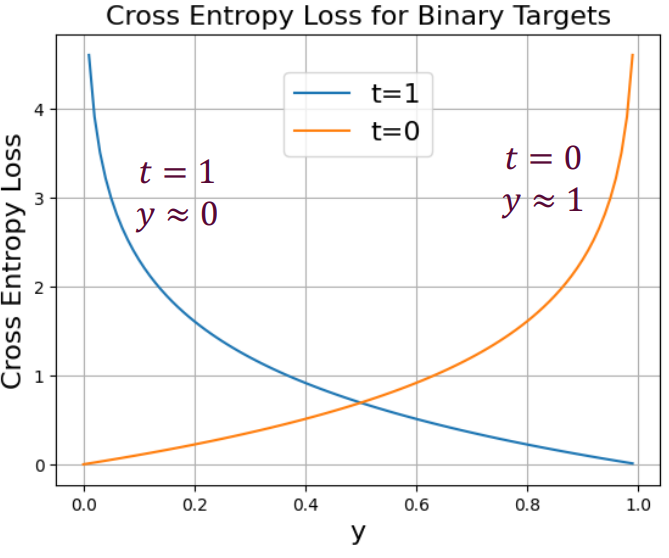
\includegraphics[width=0.45\linewidth]{ce_loss.png}

\subsection{Cross-Entropy Loss Equations}
\textbf{Linear model}
\[ z = \vw^T\vx \]
\textbf{Classification}
\begin{align*}
y &= \sigma(z) = \frac{1}{1+e^{-z}}\\
\sigma'(z) &= \sigma(z)\left(1-\sigma(z)\right)\\
\frac{\partial y}{\partial z} &= y(1-y)
\end{align*}
\textbf{Loss}
\[ \cL_{CE}(y,t) = -t\log(y) - (1-t)\log(1-y) \]
\textbf{Gradient Descent Update}\\
Where $\cE(\vw) = \frac{1}{N}\sum_{i=1}^N \cL_{CE}\left(y^{(i)}, t^{(i)}\right)$
\begin{align*}
\frac{\partial\cL_{CE}}{\partial w_j} &= \frac{\partial\cL_{CE}}{\partial y}\cdot\frac{\partial y}{\partial z}\cdot\frac{\partial z}{\partial w_j}\\
&= \left(-\frac{t}{y} + \frac{1-t}{1-y}\right)\cdot y(1-y)\cdot x_j\\
&= (y-t)x_j
\end{align*}
\textit{Tip: re-use variables, don't sub all!}\\
The gradient descent update for logistic regression is:
\begin{align*}
w_j &\leftarrow w_j - \alpha\frac{\partial\cE}{\partial w_j}\\
&= w_j - \frac{\alpha}{N}\sum_{i=1}^N\left(y^{(i)} - t^{(i)}\right)x_j^{(i)}
\end{align*}
\[ \vw \leftarrow \vw - \tfrac{\alpha}{N}X^T(\sigma(X\vw)-\vt) \]
CE: $\cL\to\infty$ for confident wrong; $\partial\cL/\partial z=y-t$ (no saturation); Convex in $\vw$; Max-likelihood. Sigmoid+SE: $\partial\cL/\partial z=(y-t)y(1-y)\approx0$ when very wrong.\\
\textbf{Boundary}: $y=0.5\iff z=\vw^T\vx=0$ (hyperplane); Class 1 where $z\ge0$.

\subsection{Softmax Regression ($K\ge3$)}
\textbf{Target} one-hot $\vt\in\{0,1\}^K$ (1 at true class). Not integers: imply order + distance, renumbering changes model; One-hot: no order, all pairs equidistant.\\
\textbf{Logits} $\mathbf z=W\vx\in\mathbb R^K$, $W\in\mathbb R^{K\times(D+1)}$, row $k=[b_k,\vw_k^T]$, $z_k=\vw_k^T\vx$ (unnormalized). Predict $\arg\max_k z_k$.
\[ y_k=\tfrac{\exp(z_k)}{\sum_{k'=1}^K\exp(z_{k'})},\quad \mathbf{y}=\text{softmax}(\mathbf z)\in\mathbb R^K \]
\textbf{Properties}: (1) prob.\ dist.: $y_k\in(0,1)$, $\sum_k y_k=1$. (2) order-preserving ($\because\exp\uparrow$) $\Rightarrow\arg\max y=\arg\max z$, softmax doesn't change boundary; $y_k$ = confidence. (3) smooth, differentiable approx.\ of argmax $\Rightarrow$ GD works. (4) $K=2$: $y_1=\frac{e^{z_1}}{e^{z_1}+e^{z_2}}=\frac{1}{1+e^{-(z_1-z_2)}}=\sigma(z_1\!-\!z_2)$, $y_2=\sigma(-z)$.\\
\textbf{Loss} $\cL_{CE}=-\sum_k t_k\log y_k=-\vt^T\log\mathbf{y}=-\log y_{\text{true}}$ (1 nonzero term).\\
\textbf{Grad} $\frac{\partial\cL}{\partial z_k}=y_k-t_k$, $\nabla_{\vw_k}\cL=(y_k-t_k)\vx$
\[ \vw_k\leftarrow\vw_k-\tfrac{\alpha}{N}\textstyle\sum_i(y_k^{(i)}-t_k^{(i)})\vx^{(i)} \]
Matrix: $\nabla_W\cE=\frac1N(Y-T)^TX$ ($Y,T\in\mathbb R^{N\times K}$, rows $\mathbf{y}^{(i)T},\vt^{(i)T}$).\\
\textbf{Boundary $i$/$j$} needs BOTH: (1) $z_i=z_j\iff(\vw_i-\vw_j)^T\vx=0$ (line); (2) $z_k\le z_i\ \forall k\ne i,j$.\\
\textit{Steps}: solve (1) for line $\to$ substitute into (2) $\to$ inequality gives ray/segment $\to$ all 3 lines meet where $z_1=z_2=z_3$ $\to$ test pt per region. At most $K(K\!-\!1)/2$ boundaries.\\
Linear boundaries, convex regions; Can't do nonlinear.

\end{multicols*}
\end{document}
